% inkscape gosper.pdf --export-type=png --export-filename=gosper.png --export-width=1024 --export-background-opacity=0
% \documentclass[a3paper]{article}
% \usepackage[left=0mm,top=1cm,right=0mm,bottom=0mm]{geometry}
\documentclass[border=0]{standalone}
% \documentclass[dvisvgm]{minimal}
\usepackage{tikz}
\usetikzlibrary{calc,lindenmayersystems}
\usepackage{xcolor}
\definecolor{pGreen}{HTML}{663366}
\pgfdeclarelindenmayersystem{Gosper}{
\symbol{A}{\pgflsystemdrawforward}
\symbol{B}{\pgflsystemdrawforward}
\symbol{+}{\pgflsystemturnright} % Explicitly define + and - symbols.
\symbol{-}{\pgflsystemturnleft}
\rule{A -> A-B--B+A++AA+B-}
\rule{B -> +A-BB--B-A++A+B}
}
\begin{document}
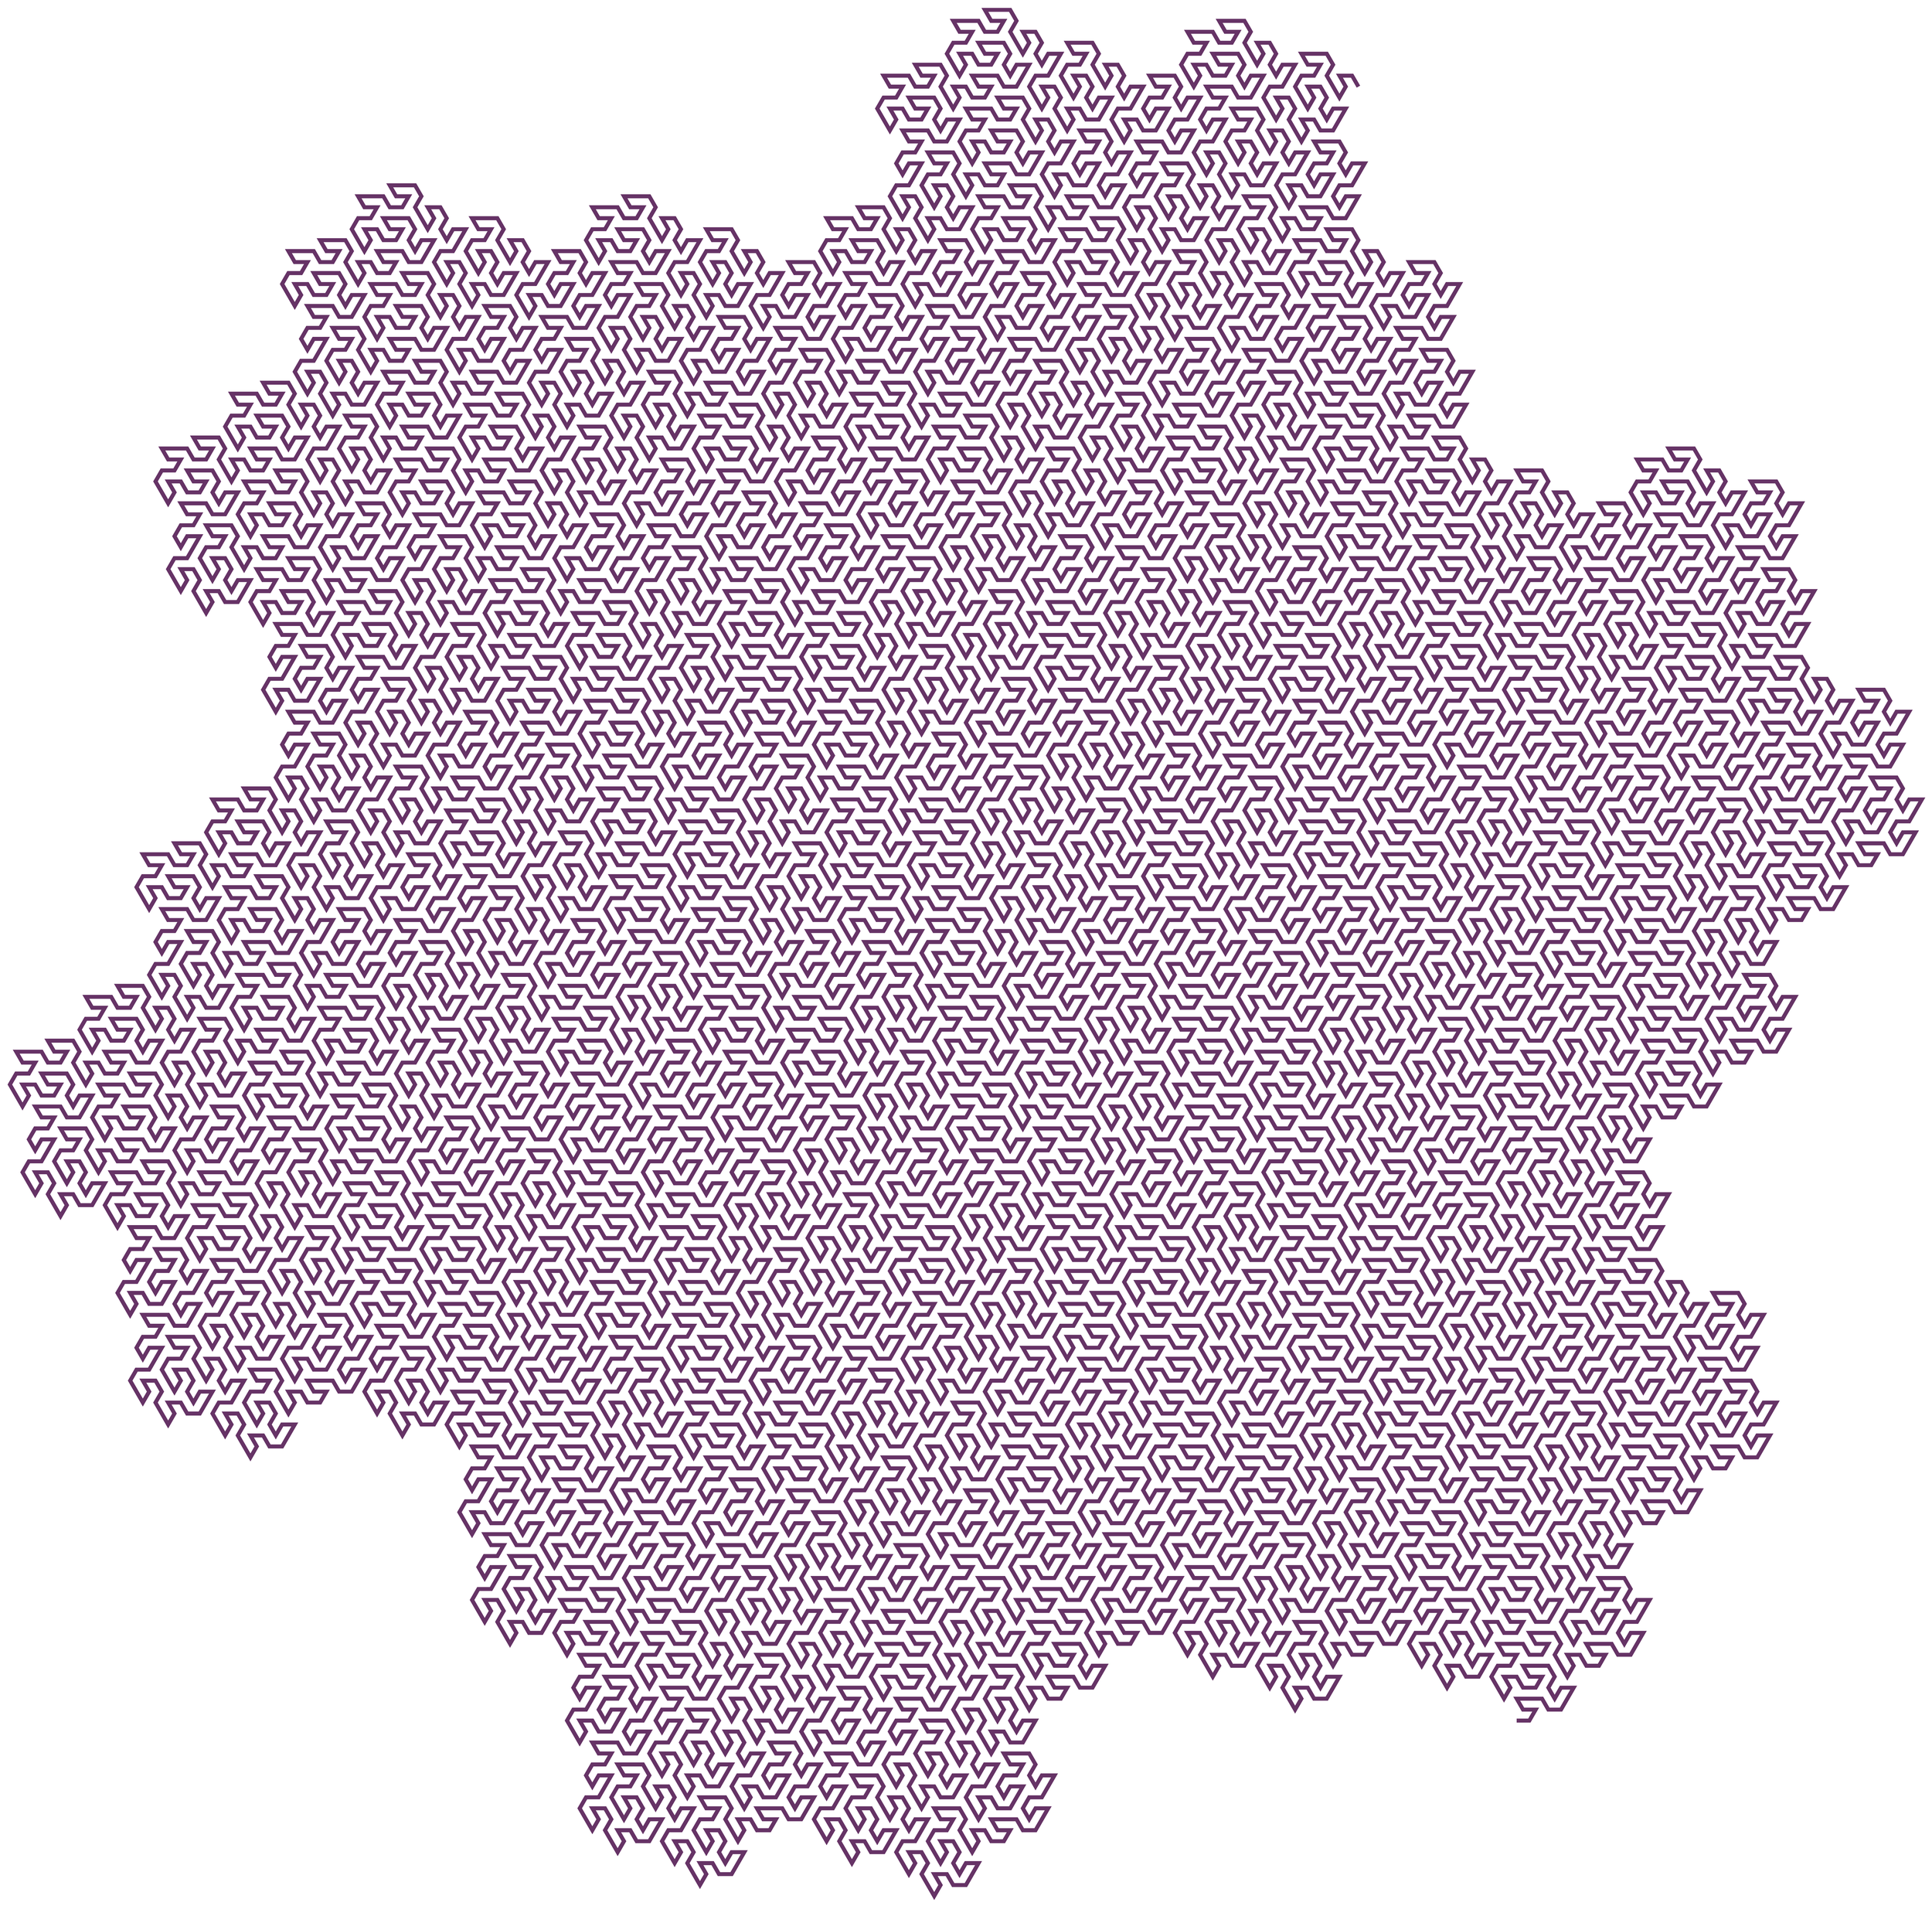
\begin{tikzpicture}
      \draw[lindenmayer system={Gosper, step=16, axiom=A, order=5, angle=60},pGreen,line width=5pt] lindenmayer system;
\end{tikzpicture}
\end{document}